\documentclass[twoside]{book}

% Packages required by doxygen
\usepackage{fixltx2e}
\usepackage{calc}
\usepackage{doxygen}
\usepackage{graphicx}
\usepackage[utf8]{inputenc}
\usepackage{makeidx}
\usepackage{multicol}
\usepackage{multirow}
\PassOptionsToPackage{warn}{textcomp}
\usepackage{textcomp}
\usepackage[nointegrals]{wasysym}
\usepackage[table]{xcolor}

% Font selection
\usepackage[T1]{fontenc}
\usepackage{mathptmx}
\usepackage[scaled=.90]{helvet}
\usepackage{courier}
\usepackage{amssymb}
\usepackage{sectsty}
\renewcommand{\familydefault}{\sfdefault}
\allsectionsfont{%
  \fontseries{bc}\selectfont%
  \color{darkgray}%
}
\renewcommand{\DoxyLabelFont}{%
  \fontseries{bc}\selectfont%
  \color{darkgray}%
}
\newcommand{\+}{\discretionary{\mbox{\scriptsize$\hookleftarrow$}}{}{}}

% Page & text layout
\usepackage{geometry}
\geometry{%
  a4paper,%
  top=2.5cm,%
  bottom=2.5cm,%
  left=2.5cm,%
  right=2.5cm%
}
\tolerance=750
\hfuzz=15pt
\hbadness=750
\setlength{\emergencystretch}{15pt}
\setlength{\parindent}{0cm}
\setlength{\parskip}{0.2cm}
\makeatletter
\renewcommand{\paragraph}{%
  \@startsection{paragraph}{4}{0ex}{-1.0ex}{1.0ex}{%
    \normalfont\normalsize\bfseries\SS@parafont%
  }%
}
\renewcommand{\subparagraph}{%
  \@startsection{subparagraph}{5}{0ex}{-1.0ex}{1.0ex}{%
    \normalfont\normalsize\bfseries\SS@subparafont%
  }%
}
\makeatother

% Headers & footers
\usepackage{fancyhdr}
\pagestyle{fancyplain}
\fancyhead[LE]{\fancyplain{}{\bfseries\thepage}}
\fancyhead[CE]{\fancyplain{}{}}
\fancyhead[RE]{\fancyplain{}{\bfseries\leftmark}}
\fancyhead[LO]{\fancyplain{}{\bfseries\rightmark}}
\fancyhead[CO]{\fancyplain{}{}}
\fancyhead[RO]{\fancyplain{}{\bfseries\thepage}}
\fancyfoot[LE]{\fancyplain{}{}}
\fancyfoot[CE]{\fancyplain{}{}}
\fancyfoot[RE]{\fancyplain{}{\bfseries\scriptsize Generated on Sun Jan 25 2015 20\+:16\+:31 for My Project by Doxygen }}
\fancyfoot[LO]{\fancyplain{}{\bfseries\scriptsize Generated on Sun Jan 25 2015 20\+:16\+:31 for My Project by Doxygen }}
\fancyfoot[CO]{\fancyplain{}{}}
\fancyfoot[RO]{\fancyplain{}{}}
\renewcommand{\footrulewidth}{0.4pt}
\renewcommand{\chaptermark}[1]{%
  \markboth{#1}{}%
}
\renewcommand{\sectionmark}[1]{%
  \markright{\thesection\ #1}%
}

% Indices & bibliography
\usepackage{natbib}
\usepackage[titles]{tocloft}
\setcounter{tocdepth}{3}
\setcounter{secnumdepth}{5}
\makeindex

% Hyperlinks (required, but should be loaded last)
\usepackage{ifpdf}
\ifpdf
  \usepackage[pdftex,pagebackref=true]{hyperref}
\else
  \usepackage[ps2pdf,pagebackref=true]{hyperref}
\fi
\hypersetup{%
  colorlinks=true,%
  linkcolor=blue,%
  citecolor=blue,%
  unicode%
}

% Custom commands
\newcommand{\clearemptydoublepage}{%
  \newpage{\pagestyle{empty}\cleardoublepage}%
}


%===== C O N T E N T S =====

\begin{document}

% Titlepage & ToC
\hypersetup{pageanchor=false,
             bookmarks=true,
             bookmarksnumbered=true,
             pdfencoding=unicode
            }
\pagenumbering{roman}
\begin{titlepage}
\vspace*{7cm}
\begin{center}%
{\Large My Project }\\
\vspace*{1cm}
{\large Generated by Doxygen 1.8.8}\\
\vspace*{0.5cm}
{\small Sun Jan 25 2015 20:16:31}\\
\end{center}
\end{titlepage}
\clearemptydoublepage
\tableofcontents
\clearemptydoublepage
\pagenumbering{arabic}
\hypersetup{pageanchor=true}

%--- Begin generated contents ---
\chapter{Class Index}
\section{Class List}
Here are the classes, structs, unions and interfaces with brief descriptions\+:\begin{DoxyCompactList}
\item\contentsline{section}{\hyperlink{classdzialania}{dzialania} \\*Klasa dzialania }{\pageref{classdzialania}}{}
\item\contentsline{section}{\hyperlink{class_kalkulator2_1_1_form1}{Kalkulator2.\+Form1} \\*Klasa glowna }{\pageref{class_kalkulator2_1_1_form1}}{}
\item\contentsline{section}{\hyperlink{classprzelicznik}{przelicznik} \\*Klasa przelicznik }{\pageref{classprzelicznik}}{}
\end{DoxyCompactList}

\chapter{Class Documentation}
\hypertarget{classdzialania}{\section{dzialania Class Reference}
\label{classdzialania}\index{dzialania@{dzialania}}
}


Klasa dzialania.  


\subsection*{Public Member Functions}
\begin{DoxyCompactItemize}
\item 
\hypertarget{classdzialania_a5789152d0cae6fcd0efcd80a97317b7a}{double {\bfseries mnozenie} (double a, double b)}\label{classdzialania_a5789152d0cae6fcd0efcd80a97317b7a}

\item 
\hypertarget{classdzialania_a7989524b1d5dabb6f7e798c2658dfe92}{double \hyperlink{classdzialania_a7989524b1d5dabb6f7e798c2658dfe92}{dzielenie} (double a, double b)}\label{classdzialania_a7989524b1d5dabb6f7e798c2658dfe92}

\begin{DoxyCompactList}\small\item\em Funkcja mnozenia. \end{DoxyCompactList}\item 
\hypertarget{classdzialania_aedd526ca5c15cc5afa5dac56559b6d52}{double \hyperlink{classdzialania_aedd526ca5c15cc5afa5dac56559b6d52}{dodawanie} (double a, double b)}\label{classdzialania_aedd526ca5c15cc5afa5dac56559b6d52}

\begin{DoxyCompactList}\small\item\em funkcja dzielenia \end{DoxyCompactList}\item 
\hypertarget{classdzialania_a26c19288a004b2938cc41c72921d09ee}{double \hyperlink{classdzialania_a26c19288a004b2938cc41c72921d09ee}{odejmowanie} (double a, double b)}\label{classdzialania_a26c19288a004b2938cc41c72921d09ee}

\begin{DoxyCompactList}\small\item\em funkcja dodawania \end{DoxyCompactList}\item 
\hypertarget{classdzialania_a88e66bf8dc5e38da26b8beb3a7c3e268}{double \hyperlink{classdzialania_a88e66bf8dc5e38da26b8beb3a7c3e268}{pierwiastek} (double a, double b)}\label{classdzialania_a88e66bf8dc5e38da26b8beb3a7c3e268}

\begin{DoxyCompactList}\small\item\em funkcja odejmowania \end{DoxyCompactList}\item 
\hypertarget{classdzialania_af0053414eb5e56844ef90512ff48d0ac}{double \hyperlink{classdzialania_af0053414eb5e56844ef90512ff48d0ac}{potega} (double a, double b)}\label{classdzialania_af0053414eb5e56844ef90512ff48d0ac}

\begin{DoxyCompactList}\small\item\em funkcja pierwiastkowania \end{DoxyCompactList}\end{DoxyCompactItemize}


\subsection{Detailed Description}
Klasa dzialania. 

Zawiera proste operacje polegajace na dodawaniu, odejmowaniu, mnozeniu, dzieleniu oraz pierwiastkowaniu. Obsluguje liczby zmiennoprzecinkowe. 

The documentation for this class was generated from the following file\+:\begin{DoxyCompactItemize}
\item 
Kalkulator.\+cpp\end{DoxyCompactItemize}

\hypertarget{classprzelicznik}{\section{przelicznik Class Reference}
\label{classprzelicznik}\index{przelicznik@{przelicznik}}
}


Klasa przelicznik.  


Inheritance diagram for przelicznik\+:\begin{figure}[H]
\begin{center}
\leavevmode
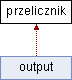
\includegraphics[height=2.000000cm]{classprzelicznik}
\end{center}
\end{figure}
\subsection*{Public Member Functions}
\begin{DoxyCompactItemize}
\item 
\hypertarget{classprzelicznik_af16918bffe6d4e2e45a498a9bb4d7344}{double {\bfseries km\+\_\+mi} (double km)}\label{classprzelicznik_af16918bffe6d4e2e45a498a9bb4d7344}

\item 
\hypertarget{classprzelicznik_a5892f14824367d5a5afe25e01b68fe13}{double {\bfseries mi\+\_\+km} (double mi)}\label{classprzelicznik_a5892f14824367d5a5afe25e01b68fe13}

\end{DoxyCompactItemize}
\subsection*{Public Attributes}
\begin{DoxyCompactItemize}
\item 
\hypertarget{classprzelicznik_acccf8fd1a56dabc8f58237eff8144e36}{double {\bfseries m} = 1.\+609344}\label{classprzelicznik_acccf8fd1a56dabc8f58237eff8144e36}

\end{DoxyCompactItemize}
\subsection*{Friends}
\begin{DoxyCompactItemize}
\item 
\hypertarget{classprzelicznik_a0a8814941837a9542fbb768e740fd03b}{class {\bfseries input}}\label{classprzelicznik_a0a8814941837a9542fbb768e740fd03b}

\end{DoxyCompactItemize}


\subsection{Detailed Description}
Klasa przelicznik. 

Zawiera proste operacje polegajace na zamianie kilometrow na mile oraz mil na kilometry 

The documentation for this class was generated from the following file\+:\begin{DoxyCompactItemize}
\item 
Kalkulator.\+cpp\end{DoxyCompactItemize}

%--- End generated contents ---

% Index
\newpage
\phantomsection
\addcontentsline{toc}{chapter}{Index}
\printindex

\end{document}
